\documentclass{sig-alternate}
%\documentclass[a4paper,10pt]{article}
\usepackage[utf8]{inputenc}
%El template pincha con spanish babel
%\usepackage[spanish]{babel}
\usepackage{graphicx}
\usepackage{fancybox}
\usepackage[table]{xcolor}
\usepackage{soul}

\title{Inventario Modelo} 

\numberofauthors{4}
\author{
\alignauthor
Pose, Alberto Miguel\\
       \affaddr{Instituto Tecnológico de Buenos Aires}\\
       \affaddr{Buenos Aires, Argentina}\\
       \email{apose@alu.itba.edu.ar}
\alignauthor
Catalano, Juan Ignacio\\
       \affaddr{Instituto Tecnológico de Buenos Aires}\\
       \affaddr{Buenos Aires, Argentina}\\
       \email{jcatalan@alu.itba.edu.ar}
\and
\alignauthor 
Palombo, Martín\\
       \affaddr{Instituto Tecnológico de Buenos Aires}\\
       \affaddr{Buenos Aires, Argentina}\\
       \email{mpalombo@alu.itba.edu.ar}
\alignauthor 
Vázquez, Santiago José\\
       \affaddr{Instituto Tecnológico de Buenos Aires}\\
       \affaddr{Buenos Aires, Argentina}\\
       \email{savazque@alu.itba.edu.ar}
}

\date{}




\begin{document}
\maketitle

\begin{abstract}
Se estudia el comportamiento del sistema correspondiente al inventario de producción de una empresa. Se plantean los modelos a lazo abierto y
lazo cerrado y se estudian condiciones de estabilidad de los mismos. Además se propone una adaptación que controla la variación de la tasa
de ventas.
\end{abstract}

\section{Introducción}
En nuestro país las huelgas a empresas se realizan mediante el abandono de las actividades correspondientes a los empleados en protesta. Por otro
lado, si observamos las huelgas en países como Japón, vemos que son totalmente contrarias a las que estamos acostumbrados. Los obreros o empleados
en lugar de suspender su actividad, sobreproducen. Esto genera un exceso de inventario en los depósitos que se torna imposible de almacenar,
resultando en una pérdida mayor para la empresa. La importancia del control de la cantidad de productos en inventario se manifiesta en este
ejemplo y es nuestra motivación principal en el estudio de este tipo de sistemas. Un antecedente a este trabajo es el realizado por I. Luciani, J. Barreira y
F. Siviero titulado ``Sistema de Control de Inventario''[1].\\ 
En la sección \ref{model_section} se presenta el modelo base utilizado para realizar la simulación. En la sección \ref{inventary_control_section} presenta una alternativa, 
agregando un set de referencia para controlar la cantidad de productos en inventario. En la sección \ref{salesrate_control_section} se controla
la tasa de ventas y se analizan los resultados obtenidos de realizar la simulación con dicho control. En la sección \ref{results_and_conclusions_section}
se presentan los resultados y conclusiones obtenidas en todo el análisis realizado para este artículo.

\section{Modelo base}
\label{model_section}

Para nuestro análisis consideramos una empresa que vende productos manufacturados los cuales son almacenados en un depósito.
El inventario de dichos bienes sigue una dinámica que cumple las siguientes propiedades:
\begin{enumerate}
\item Los productos son homogéneos. Esto permite poder realizar un mismo proceso para todos ellos.
\item La cantidad de productos manipulada en cada ejercicio es muy grande. Esta condición nos permite aproximar como continuo, este sistema de
naturaleza discreta.
\end{enumerate}
El modelo que se propone define $x_{1}(t)$ como el nivel
de inventario y $x_{2}(t)$ como la tasa de ventas del producto. Además,
se establece la velocidad de variación de la tasa de ventas como proporcional a $u(t)$, el flujo de entrada. Dicha relación queda explicitada en
\eqref{eq:la_k}.

\begin{equation}
\frac{dx_{2}}{dt}(t)=-Ku(t)\label{eq:la_k}\end{equation}


Donde K > 0.\\
Luego, definimos la velocidad de variación del inventario $\dot{x_{1}}(t)$ como se muestra en \eqref{eq:dotx1}.

\begin{equation}
\dot{x}_{1}(t)=u(t)-x_{2}(t)\label{eq:dotx1}\end{equation}

Esto significa que la variación de la cantidad de productos en inventario depende de lo
que se produce (entra) y de lo que se vende (sale). Este comportamiento se puede detallar como sigue:
\begin{enumerate}
\item Si $x_{2}<u(t)$ el nivel de inventario aumenta, $\dot{x}_{1}(t)>0$.
Esto se debe a que se produce más de lo que se vende.
\item Mientras que cuando $x_{2}(t)>u(t)$ el inventario disminuye más rápidamente que lo que se repone mediante nueva producción, 
$\dot{x}_{1}(t)<0$. Es decir, se vende más de lo que se produce.
\item Cuando $x_{2}=u(t)$, refleja que $\dot{x}_{1}(t)=0$ y la cantidad de
elementos en el inventario permanece constante. Esto puede atribuirse
a que se vende tanto como lo que se produce o a que no se vende ni
se produce ningún producto.

\end{enumerate}

Para realizar la simulación, consideramos $x_{2} = C$, una constante. Es decir, asumiendo que la tasa de ventas se mantiene fija en el tiempo.\\
El modelo planteado en esta sección se denomina a lazo abierto, ya que no se propone realimentación alguna para la entrada del sistema. 
En la figura \ref{fig:lazo_abierto} podemos observar como evoluciona en este caso la cantidad de productos para distintos valores de $K$. 
Se puede notar que al aumentarel valor de dicha constante, el depósito se vacía más rápidamente que si consideramos valores de $K$ cercanos a
cero.

\begin{figure}[h]
\begin{center}
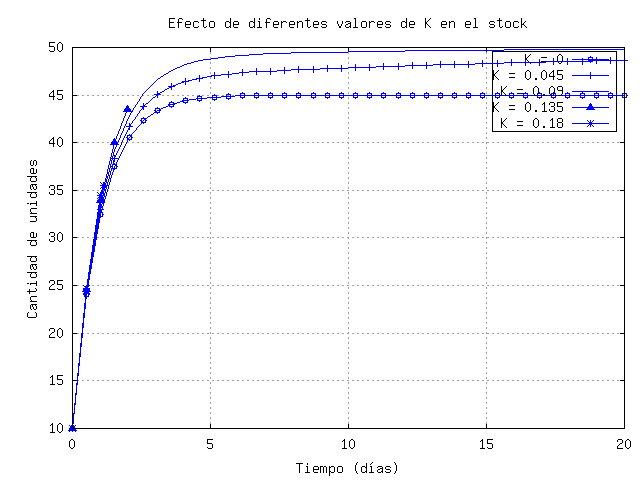
\includegraphics[width=8cm]{../src/k_plot.png}
\caption{\label{fig:lazo_abierto} }
\end{center}
\end{figure}

\section{Controlando el inventario}
\label{inventary_control_section} 
Se desea controlar el nivel del inventario tomando como output $y(t)=x_{1}(t)$ y considerando
un set point de referencia $r(t)$. Es decir, que $u(t)$ queda explicitado como se muestra en \eqref{eq:ut}.

\begin{equation}
u(t)= Ke(t) = K(r(t)-y(t))\label{eq:ut}\end{equation}
Resultando en la adaptación del modelo, ahora a lazo cerrado que se muestra en \eqref{eq:lazo_cerrado}

\begin{equation}
\dot{x}_1(t) = K(r(t) - x_{1}(t)) - C\label{eq:lazo_cerrado}\end{equation}

A fines de regular el inventario de manera tal que la cantidad de productos tienda a mantenerse constante, definimos $r(t)$ como una función
constante.
Como se puede ver, esta adaptación del modelo queda completamente controlada por la constante $K$ definida en la sección anterior. Empíricamente se llega al resultado que muestra que cuando $0.799 < K < 5.687$ el modelo se comporta de forma estable, alcanzando el comportamiento
que se desea obtener mediante la regulación impuesta. El valor alcanzado en el regimen estable
es el valor tomado como set point de referencia, en nuestro caso $r(t) = 1000$.\\
Podemos ver entonces que existe relación entre lo que se vende y lo que se produce y que dicha relación se encuentra gobernada por el valor de
$K$. La definición de dicho parámetro lleva a que el sistema sobreproduzca o no.
    % Poner más jugos con el gráfico.
    
\section{Controlando la tasa de ventas}
\label{salesrate_control_section}
Veamos de plantear una adaptación del modelo en donde se controle el variación de la tasa de ventas. Para ello proponemos una ecuación diferencial
tal que $\dot{x}_{2}$ dependa de la cantidad de productos en inventario. Esto se sustenta en la idea de que la variación de la tasa de unidades
vendidas depende de que se disponga de dichos bienes para su venta. Por ende, $\dot{x}_{2}$ resulta de la forma explicitada en \eqref{eq:x_2dot}.

\begin{equation}
 \label{eq:x_2dot}
 \frac{dx_{2}}{dt}(t) = 6x_1(t) - Ku(t)
\end{equation}
Como podemos ver, el comportamiento del modelo sigue regido por el valor de $K$. En la figura vemos que para determinados valores de $K$ el sistema
oscila inestablemente, mientras que para otros valores logra estabilizarse en el set point de referencia.\\
En la figura \ref{fig:lazo_cerrado_var_tventas} vemos como para valores de $K$ fuera del rango de estabilidad, el modelo oscila de
forma inestable y si tomamos los valores dentro de dicho rango, el modelo se comporta de manera estable. Dentro de dicho rango, aumentar el 
valor de $K$ lleva a que el sistema se estabilice en valores mayores al utilizado como referencia. Por otro lado, si utilizamos un $K$ menor podemos ver como el 
modelo se estabiliza cada vez más cercano al set point de referencia.

\begin{figure}[h]
\begin{center}
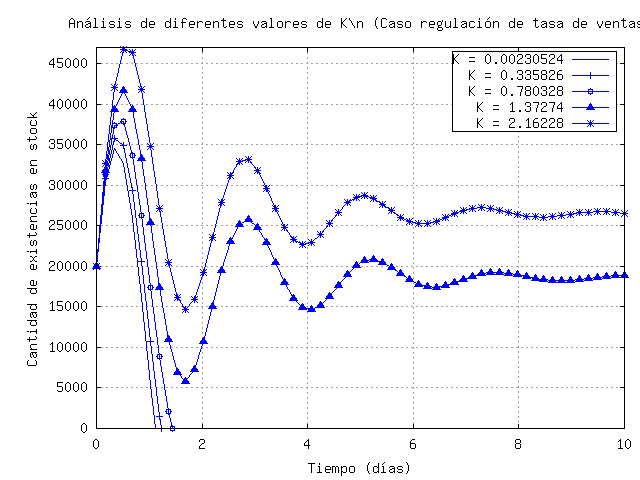
\includegraphics[width=8cm]{../src/k_plot2.png}
\caption{\label{fig:lazo_cerrado_var_tventas} }
\end{center}
\end{figure}

\section{Resultados y Conclusiones}
\label{results_and_conclusions_section}
A lo largo del trabajo se verifican los modelos tanto a lazo cerrado como lazo abierto. Se puede ver el éxito de su uso para modelar un sistema
de inventario de productos. Al variar el inventario utilizando un modelo a lazo abierto observamos como la cantidad de productos disminuye de
forma exponencial ya que no ocurre aporte alguno a la producción.  Por otro lado, en el modelo a lazo cerrado, vemos como la producción 
incrementa hasta llegar al valor que se fijó como referencia. En este caso el valor de $K$ también es fundamental ya que determina
en que cantidad de productos se desvía inicialmente la producción antes de estabilizarse. Además, al controlar la variación de la tasa de ventas,
el valor de $K$ determina la cantidad de productos en que se estabiliza el sistema. Para valores más cercanos a cero, se aproxima al punto
elegido como referencia. Al aumentarlo, el punto en el que se estabiliza disminuye.

\bibliographystyle{plain}
\nocite{*}
\bibliography{references}

\end{document}
